\section{Theorie}
\label{sec:Theorie}
\subsection{Austrittsarbeit und Energieverteilung von Elektronen}
Metalle sind kristalline Festkörper. Sie bilden ein Gitter von 
ionisierten Atomen, welches von nahezu kräftefrei bewegten Elektronen 
eingehüllt wird. Kräftefrei ist es da im Inneren des Metalles das "Gitterpotential"
nahezu konstant ist. Demnach können sich die Elektronen dort frei bewegen. Um Elektronen jedoch 
aus dem Metall zu emittieren, muss eine Austritsarbeit überwunden werden, da das Potential außerhalb 
des Metalls verschieden ist.
\begin{figure}[H]
    \centering
        \centering
        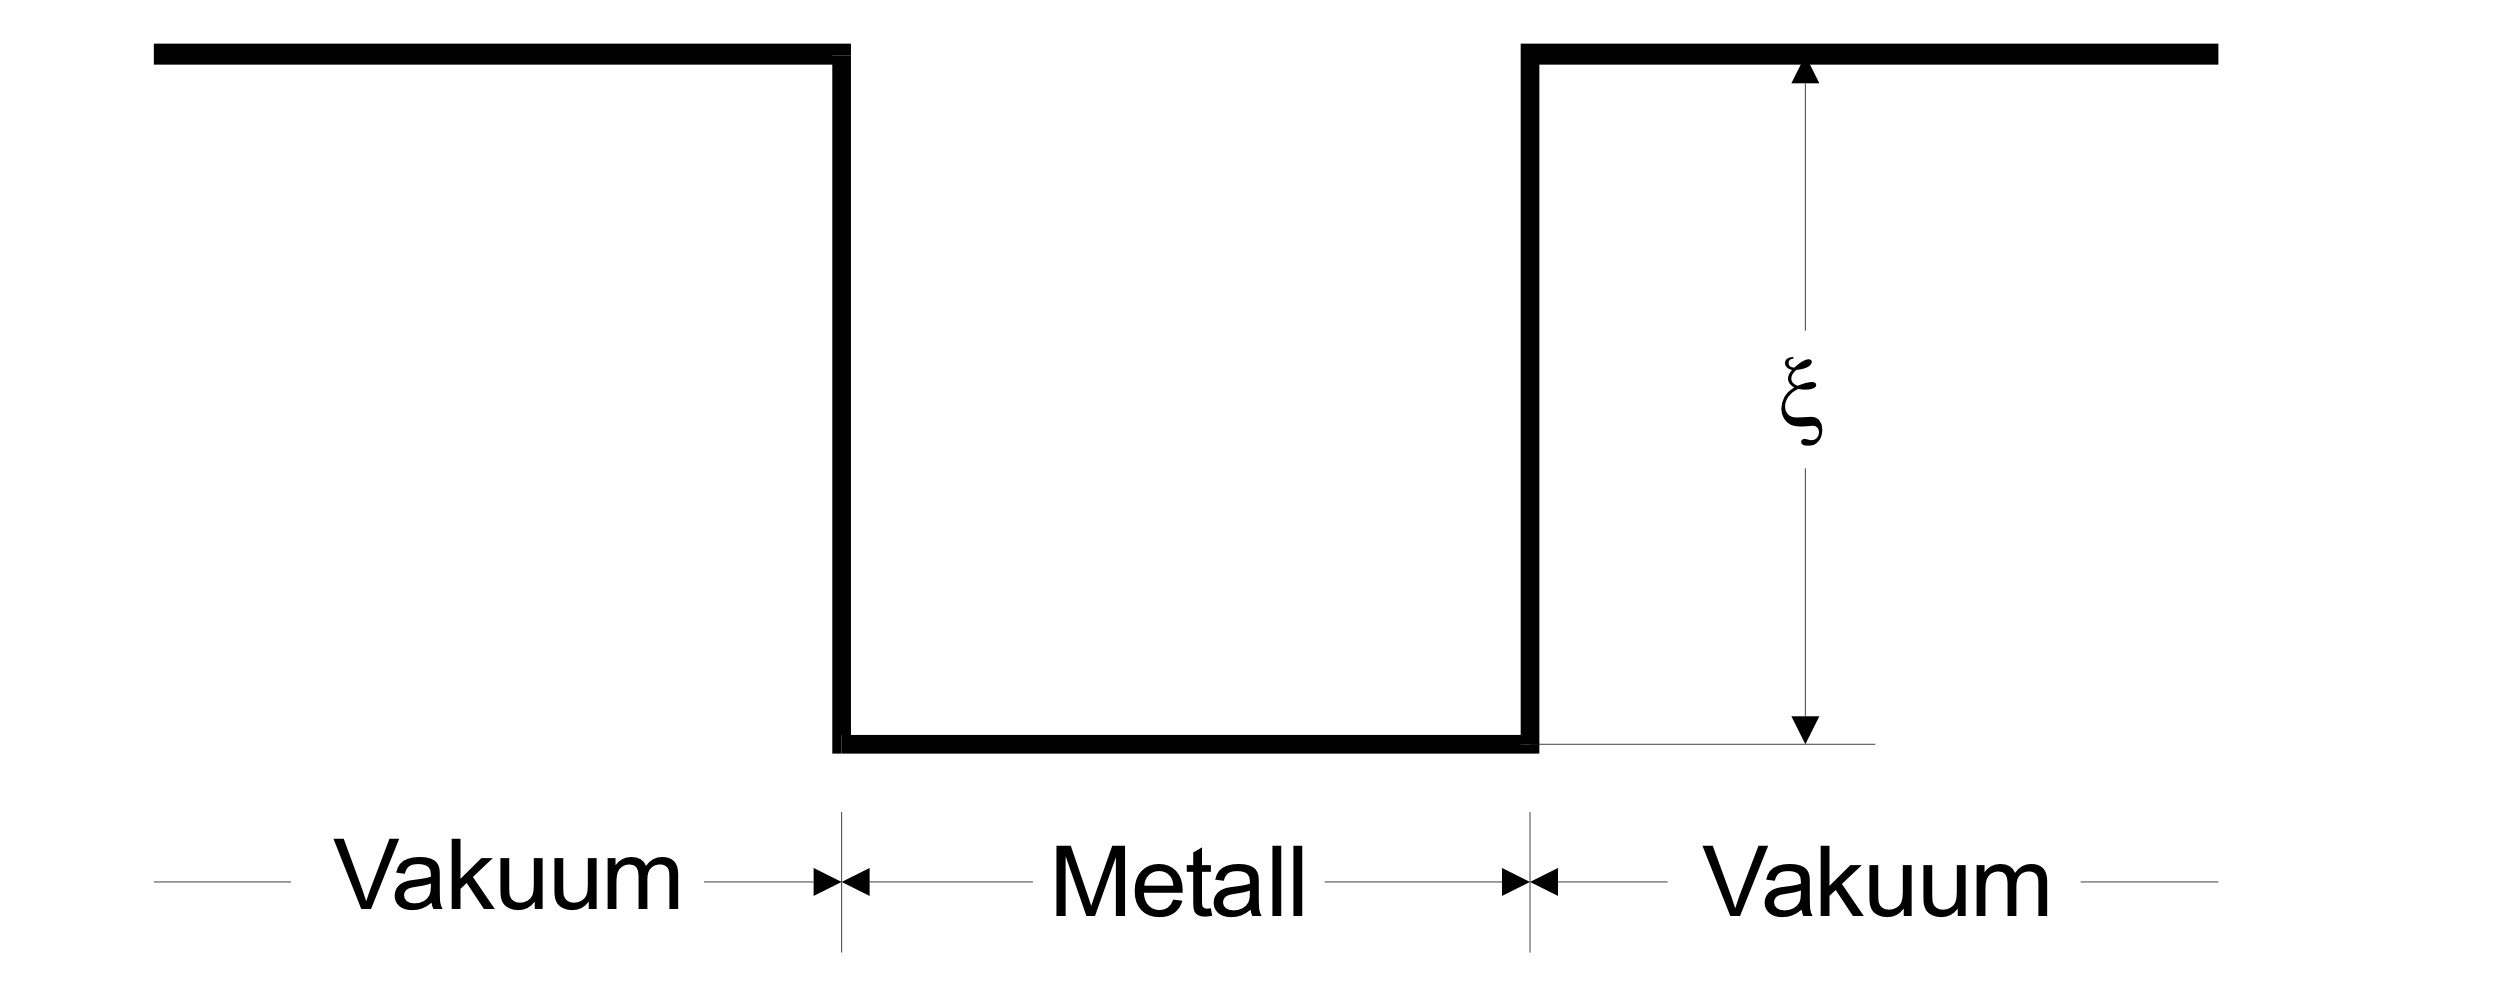
\includegraphics[width=\textwidth]{Bilder/potentialtopf.jpg}
        \caption{Potentialtopf-Modell eines Metalls. \cite{anleitung4}}
    \hfill
    \label{fig:phasendiagramm}
\end{figure}
\noindent Anhand des Potentialtopfmodells lässt sich verdeutlichen, dass die Elektronen eine 
Austritsarbeit von $\exp e_0 \xi$ verrichten müssen.
\noindent Elektronen unterliegen dem Pauli Prinzip: Das bedeutet, dass nur Elektronen mit
entgegengesetzten Spinstellungen einen möglichen Zustand besetzen können.
Folglich wird die Energieverteilung der Elektronen in einem Metall durch die Fermi-Dirac Verteilung
beschrieben.
\begin{equation}
    \label{eqn:1}
    f\left(E\right) = \frac{1}{\exp{\frac{\zeta-E}{k_b T} + 1}}
\end{equation}
\noindent In \autoref{eqn:1} ist die Fermi-Dirac Verteilungsfunktion mit der Fermi-Energie
$\zeta$ gegeben. Diese kann für eine hohe Energie $\zeta$, welche die Austritsarbeit überwinden kann,
genähert werden. die Näherung ist in \autoref{eqn:2} 
gegeben. Des weiteren ist der Verlauf der Verteilungsfunktion in \autoref{fig:fermi} dargestellt.
\begin{equation}
    \label{eqn:2}
    f\left(E\right) \approx \exp{\frac{\zeta-E}{k_b T}}
\end{equation}
\begin{figure}[H]
    \centering
        \centering
        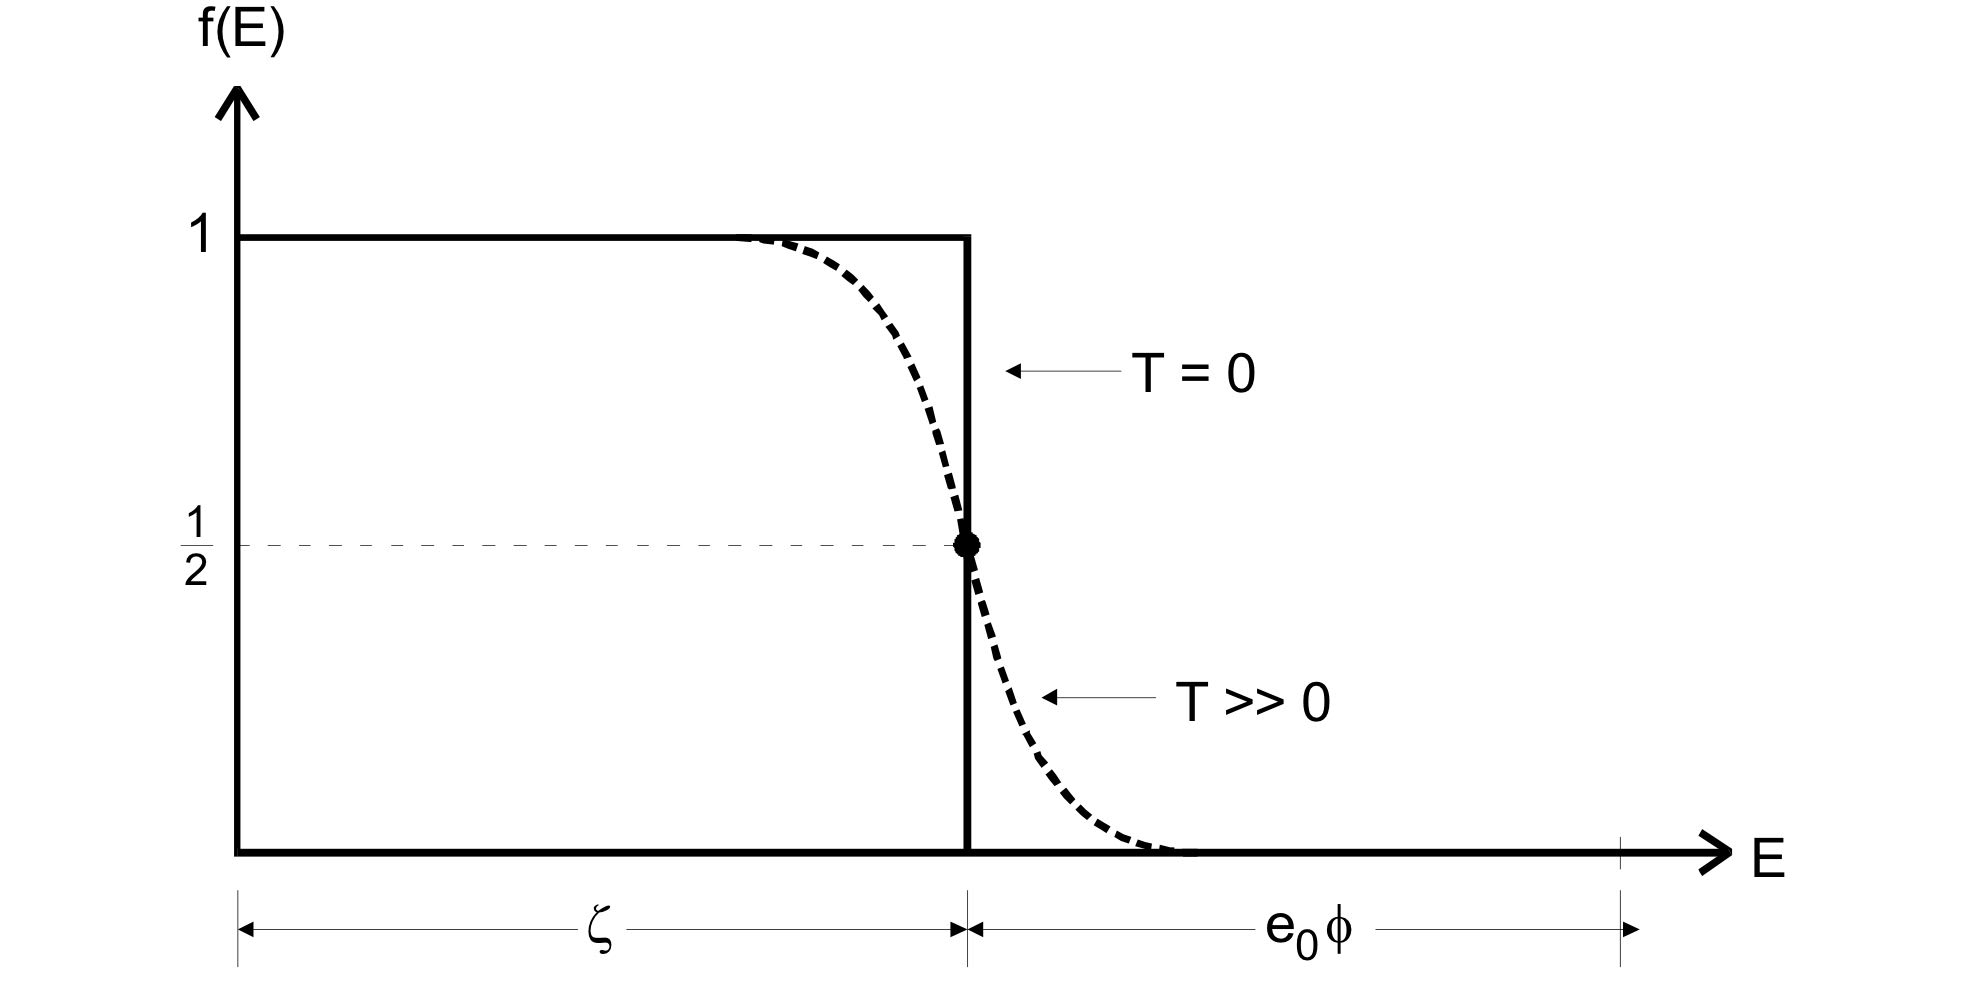
\includegraphics[width=\textwidth]{Bilder/Fermi-Dirac.jpg}
        \caption{Fermi-Dirac Verteilung. \cite{anleitung4}}
    \hfill
    \label{fig:fermi}
\end{figure}

\subsection{Sättigungsstromdichte der thermischen Elektronenemission}
Aus \autoref{eqn:2} lässt sich die Anzahl der pro Zeit austretenden Elektronen
ableiten. Diese ist temperaturabhängig und wird durch die Richardson-Gleichung
in \autoref{eqn:3} beschrieben.
\begin{equation}
    \label{eqn:3}
    j_s \left(T\right) = 4\pi \frac{e_0m_0k_B^2}{h^3}T^2\exp{-\frac{e_0\Phi}{k_b T}}
\end{equation}

\subsection{Die Hochvakuum-Diode und Langmuir-Schottkysche Raumladungsgleichung}
\label{sec:refdufotze}
Um die austretenden Elektronen zu messen, muss das Metall in ein Vakuum gebracht
werden. Damit werden Wechselwirkungen von Elektronen mit Gasmolekülen vorgebeugt. 
Im Vakuum können sie durch ein angelegtes Spannungsfeld zu einer Anode abgesaugt
werden. Es kommt eine Hochvakuumdiode wie in \autoref{fig:f10} zum Einsatz.
\begin{figure}[H]
    \centering
        \centering
        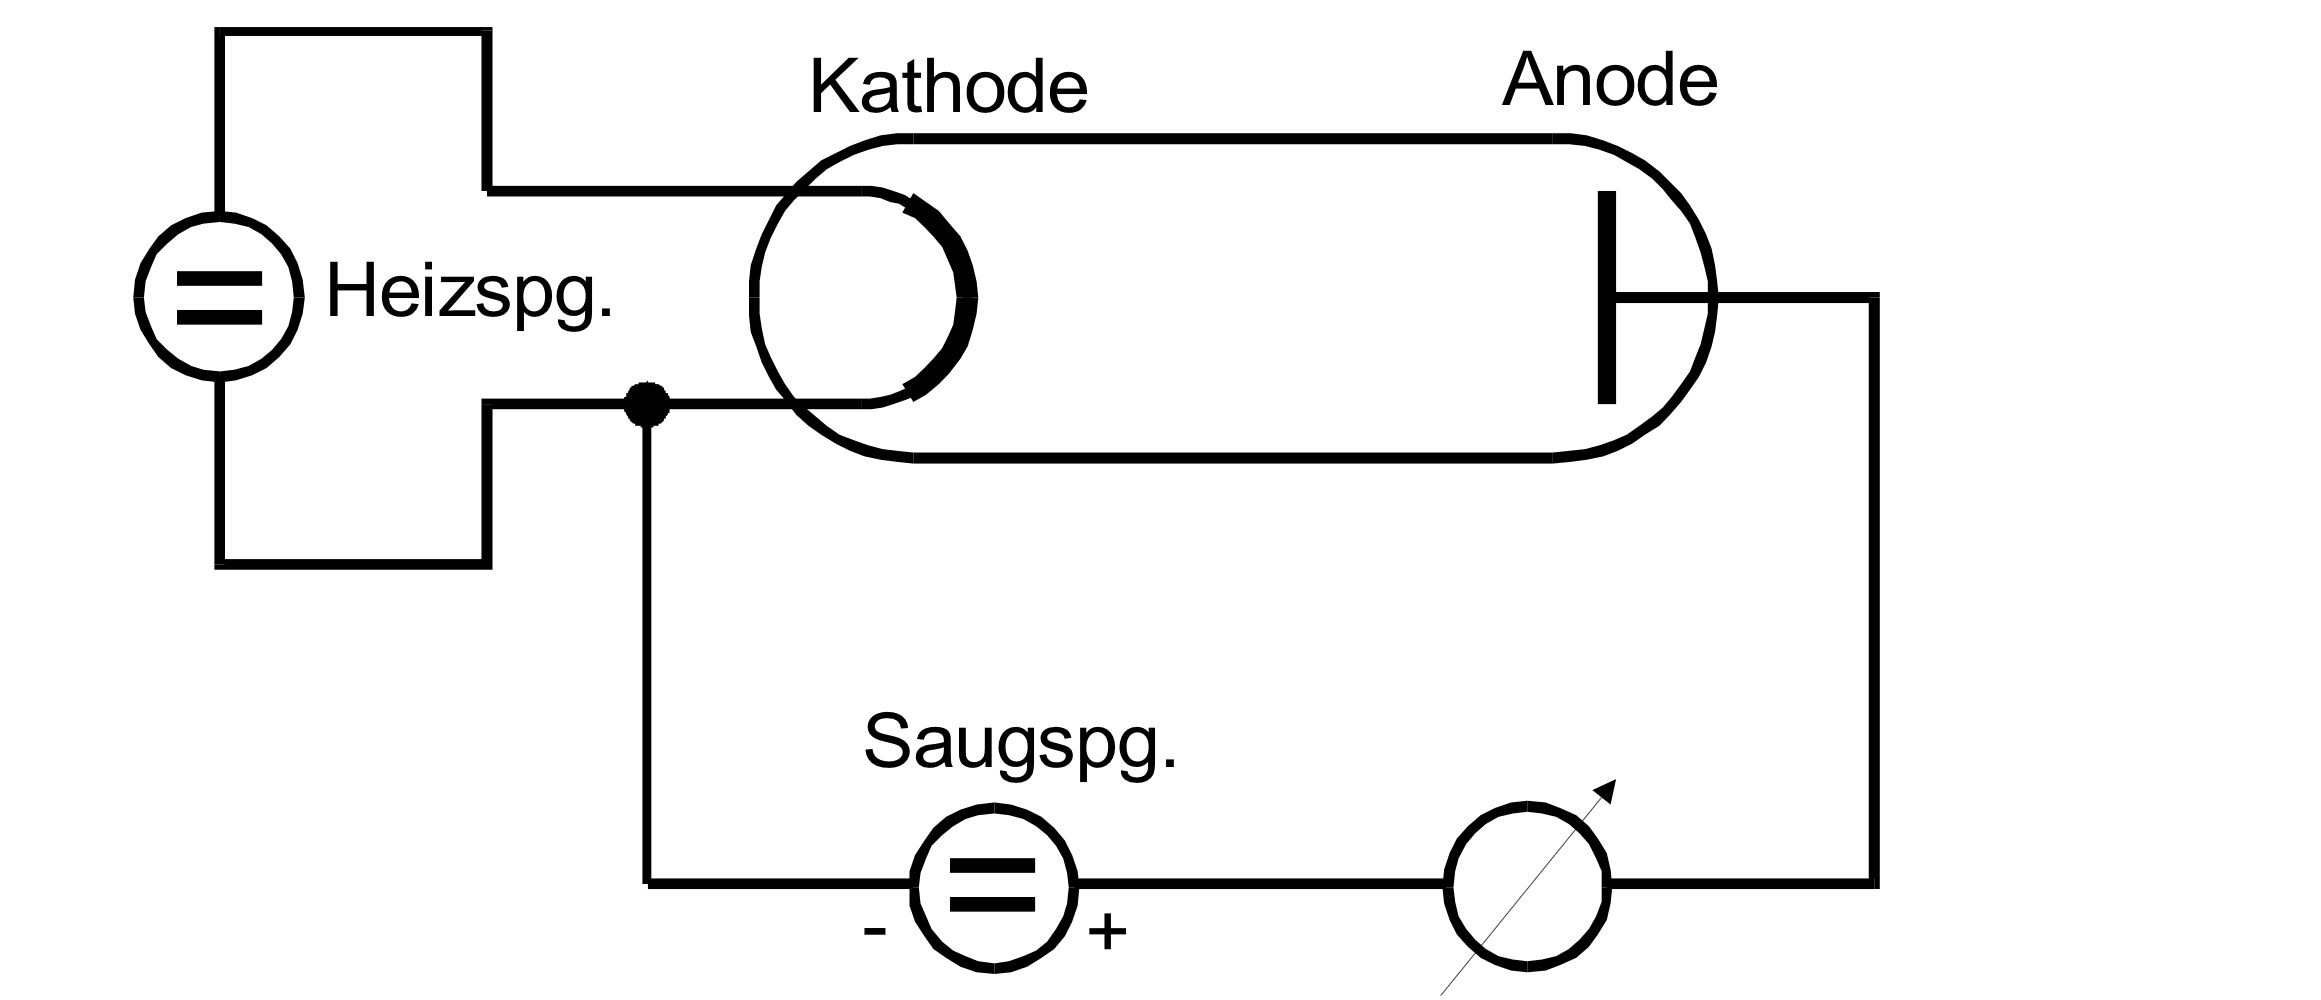
\includegraphics[width=\textwidth]{Bilder/schaltung.jpg}
        \caption{Schaltung einer Hochvakuum-Diode. \cite{anleitung4}}
    \hfill
    \label{fig:f10}
\end{figure}
\noindent Durch das elektrische Feld der positiv geladenen Anode werden die Elektronen
beschleunigt, wobei ihre Geschwindigkeit mit abnehmendem Abstand zur Anode
zunimmt. Dadurch haben eine höhere Geschwindigkeit je näher sie
der Anode kommen. Die Kontinuitätsbedingung der Stromdichte, 
\begin{equation}
j = -\rho v
\end{equation}
mit der Stromdichte $j$ und der Raumladungsdichte $\rho$, führt nun zu einer
unterschiedlichen Geschwindigkeitsverteilung der Elekrtonen und damit auch zu
einer Ladungsverteilung, welche von der Kathode hin zur Anode abnimmt. Durch
die unterschiedliche Ladungsdichte wird die Kathode abgeschirmt. Folglich erreichen 
nicht mehr alle Feldlinien ausgehend von der Anode, die Kathode. Damit ist der
gemessene Diodenstrom kleiner als der erwartete Sättigungsstrom.

\subsection{Kathodentemperatur}
\label{sec:kattemp}
Die Kathodentemperaturen werden über die Leistungsbilanz ermittelt. Mit dem 
Energiesatz und den Identitäten für die zugeführte Leistung $N_zu$ und dem 
Stefan-Boltzmannschen Gesetz ($N_W$), welches die Wärmestrahlung festlegt,
ergibt sich:
\begin{align*}
                         N_{zu} &= N_W + N_{WL} \\
    \Longleftrightarrow U_H I_H &= f \eta \sigma T^4 + N_{WL} \\
    \Longleftrightarrow       T &= \left(\frac{I_H U_H - N_{WL}}{f \eta \sigma}\right)^{1/4}
\end{align*}

\subsection{}

\subsection{Fehlerrechnung}
Die gemessenen Werte unterliegen Messunsicherheiten und werden demnach im
Folgenden nicht als fehlerfrei angesehen. Die Fehler entstehen bei der
Bildung der Mittelwerte durch den Fehler des Mittelwerts und bei der
Regressionsrechnung sowie der Fehlerforpflanzung durch Python.
Der Fehler des Mittelwerts ist gegeben durch 
\begin{equation}
    \begin{aligned}
        \increment \overline{x} &= \sqrt{\overline{x^2\kern-0.1em} - \overline{x}^2} \\
                            &= \frac{\sqrt{\frac{1}{N-1} \sum\limits_{i=1}^N (x_i - \overline{x})^2}}{\sqrt{N}}.
    \end{aligned}
\end{equation}

Um Fehler einzubeziehen, wird die Gauß'sche Fehlerfortpflanzung verwendet:
\begin{equation}
    \label{eqn:9}
    \increment f = \sqrt{\left(\frac{\partial f}{\partial x}\right)^2 \cdot \left(\increment x\right)^2 + \left(\frac{\partial f}{\partial y}\right)^2 \cdot \left(\increment y\right)^2 + .... + \left(\frac{\partial f}{\partial z}\right)^2 \cdot \left(\increment z\right)^2}
\end{equation}